\documentclass[aps,pre,superscriptaddress,twocolumn,longbibliography]{revtex4-2}


% Common Package References
\usepackage{graphicx}
\usepackage{dcolumn}
\usepackage{bm}
\usepackage{epstopdf}
\usepackage{algorithm}
\usepackage{algpseudocode}
\usepackage[colorlinks]{hyperref}
\usepackage{amsmath,amsthm,amssymb}
\usepackage{float}
\usepackage{epsfig}
\usepackage{mathrsfs}
\usepackage{multirow}
\usepackage[all]{xy}
\usepackage{pbox}
\usepackage{verbatim}
\usepackage{braket}
\usepackage{mathtools}
\usepackage{tikz}
\usepackage{xcolor}
\usepackage{xfrac}
\usepackage{cleveref}

% Commenting commands

% Template below: replace 'initials' with your initials
%\newcommand{\initials}[1]{{\color{magenta}{\bf [INITIALS: #1]}}}


% Custom Commands
\newcommand{\singlefigure}{0.45\textwidth}


\begin{document}

% TITLE
\title{PRL GitHub Template}

% AUTHORS
\author{John Doe}
\email{john.doe@nottingham.ac.uk}
\affiliation{School of Physics and Astronomy, University of Nottingham, Nottingham, NG7 2RD, UK}
\author{Jane Doe}
\email{jane.doe@nottingham.ac.uk}
\affiliation{School of Physics and Astronomy, University of Nottingham, Nottingham, NG7 2RD, UK}

\date{\today}

\begin{abstract}
Write your abstract here, in plain text. This will get directly input into the main.tex file. % Loads the abstract.tex file
\end{abstract}

\maketitle

% SECTIONS
% Each section is written in a different file
\section{Introduction}

Write your introduction here. One can cite\cite{ARXIVEXAMPLE} referenced in the \textit{references.bib} file.
\section{Results}

Here, one can display figures, such as in \Cref{fig:example}.

\begin{figure}
    \centering
    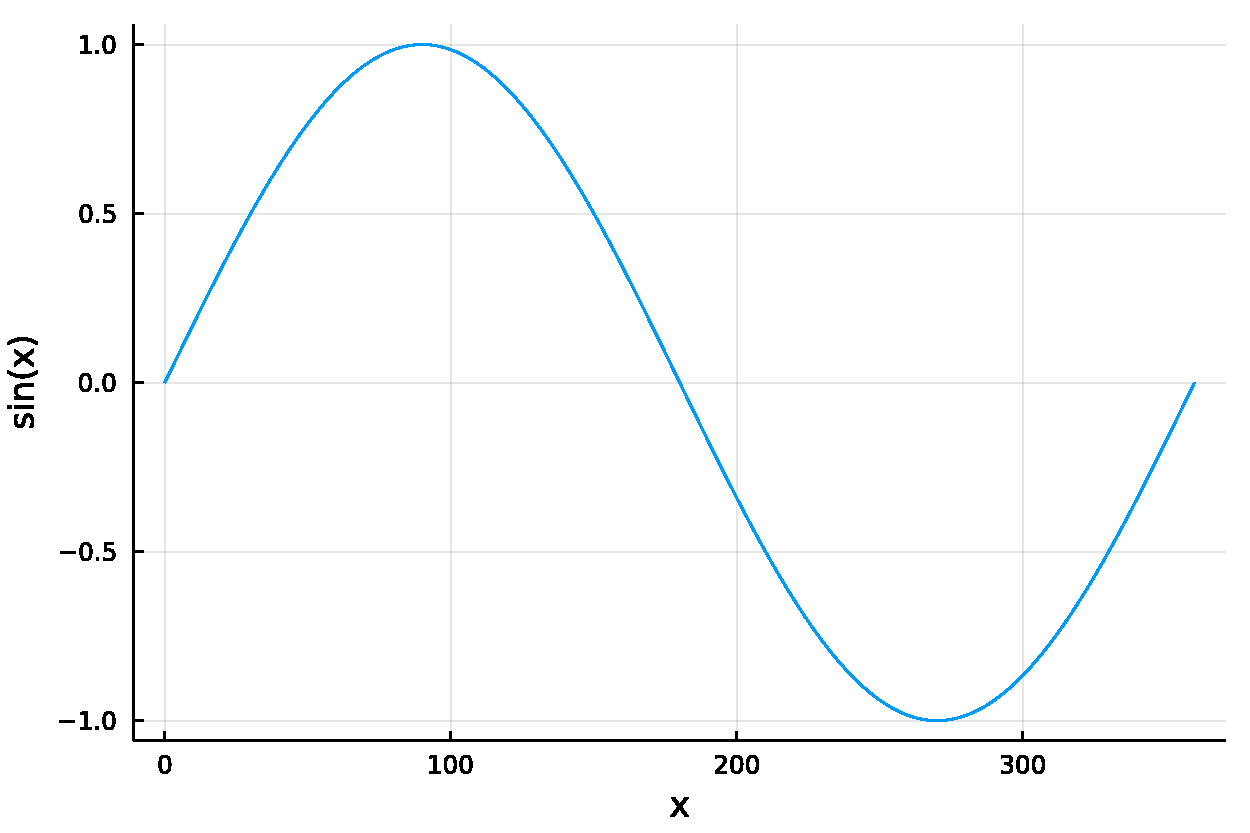
\includegraphics[width=\singlefigure]{figures/example.pdf}
    \caption{\label{fig:example} Shows an example of a figure.}
\end{figure}
\section{Conclusions}

Write your conclusions here.

% BIBLIOGRAPHY
\appendix
\bibliography{references}

\end{document}